\section{Digital Contact Tracing}

\paragraph{Goals}
\textit{Complement} manual contact tracing an a pandemic.
Notify users that they have been exposed to a person that tested positive (close than 2m for longer than 15min).
In a timely, scalable, cross-border, yet secure and privacy-preserving manner.
Using existing technologies and existing devices.

\begin{figure}[h]
	\centering
	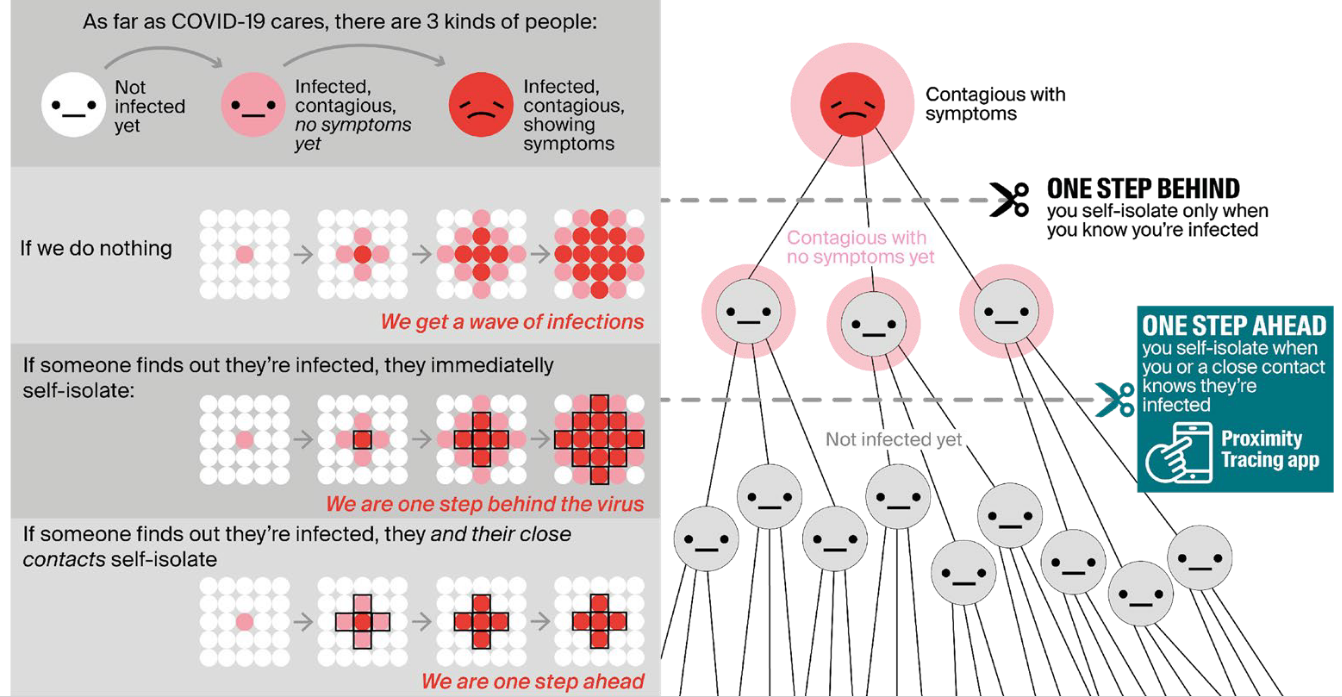
\includegraphics[scale=0.45]{images/11-why-tracing.png}
	\caption{Contact Tracing: Motivation}
	\label{fig:why-tracing}
\end{figure}

\paragraph{Exposure Notification}
Deployed by Apple and Google. Inspired by \href{https://github.com/DP-3T/documents}{DP-3T}. Used by many countries.

\underline{Idea:}
Phones broadcast ephemeral BLE\footnote{Bluetooth Low Energy} beacons.
Neighbours record beacons.
When infected, phone uploads the beacons to a public board.
Phones poll the public board.

\paragraph{DP-3T}
See the \href{https://github.com/DP-3T/documents/blob/master/DP3T\%20White\%20Paper.pdf}{white paper here}.

\paragraph{Open questions}
More evidence is needed in some of the following areas:
\begin{itemize}
	\item How reliable is Bluetooth at estimating proximity?
	\item How reliable are users to respond to a notification or trigger one?
	\item What is the financial impact of self-isolating in response to a notification?
	What demographics are more likely to comply?
	\item Access to smartphones, digital exclusion of certain groups.
	\item Is digital contact tracing a decisive factor?
	\item Inherent security\footnote{Relay+replay attacks, etc.} and privacy issues\footnote{E.g. if you only met a single person in two weeks and receive a notification, you can reliably de-anonymise them.
	However, contrast digital (privacy preserving) contact tracing with the data accumulated in manual contact tracing.}
	\item Public communication, building trust.
\end{itemize}

